% compiling and viewing latex in os x
% brew cask install mactex
% /Library/TeX/texbin/pdflatex main.tex 

\documentclass{article}
\usepackage[utf8]{inputenc}
\usepackage{listings}
\usepackage{float}
\title{Hoot de-centralized censorship free open source Live Streaming Protocol and Marketplace Technical Whitepaper}
\author{Hoot Author}
\date{July 26 2017}
\setlength{\parskip}{1em}
\usepackage{natbib}
\usepackage{graphicx}
\usepackage{amssymb}
\usepackage{amsmath}
\usepackage[normalem]{ulem}
% \usepackage{soul}
 
\begin{document}

\maketitle

\begin{abstract}
The Hoot team is building the next generation technology for live
Streaming services based on blockchain technology and a new
innovative open source de-centralized live streaming protocol that would completely eliminate expensive content delivery networks and use  peer-to-peer networks for delivering not just live streaming video but also archived videos.

\sout{We will use crypto-financing (Initial Coin Offering) for capital rather than traditional venture capital and shareholders.}

\end{abstract}
\newpage

\tableofcontents
\newpage

\section{Introduction}
Introduction for Hoot


\section{Mission}
Hoot Mission

\section{Vision}
Hoot Vision

\section{ERC223 Compatibility}
We are monitoring the ERC223 token standard proposal\footnote{https://github.com/ethereum/EIPs/issues/223} and are factoring future compatibility into the design of our Namespace Hoot tokens.

\section{What makes Hoot special}
Hoot special

\subsection{Problem \& solution}
Unfettered, censorship free live streaming

\section{Traction \& Usage}
table/ graph of usage with GB etc

\section{Low Latency Streaming Technology}
How hoot powers low latency streaming.

\section{Hoot Architecture}

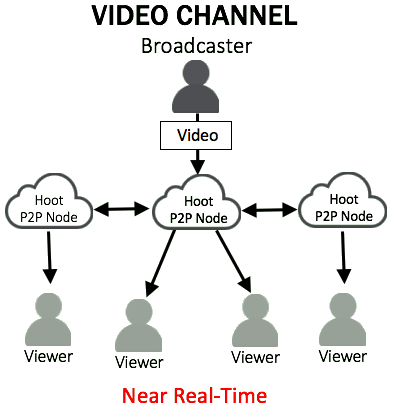
\includegraphics[scale=0.5]{static/hoot-video-architecture-channel-trans}

\subsection{Broadcast Side - mobile iOS client}
The protocol for realtime livestreaming video is called Real-Time Satoshi Streaming Protocol[\textbf{RTSSP}].
Video frames are captured at a resolution of 540x960 to 720x1280 based on network connectivity. Audio stream is captured using the built in iOS device microphone at a sampling rate of 44.1 KHz. Optionally, real time filters (Black and White, Glow, Fisheye, Sepia) can be applied to captured video frames in real-time. Video and audio are encoded using the native hardware H.264(H.265 in android) and AAC encoders, respectively. The video frames are encoded using a VBR algorithm with a maximum bitrate of 1 Mbps, this can be increased for usecases such as VR streaming. Audio stream is encoded in AAC format with a bitrate of 128 Kbps. The H.264 + AAC stream is encoded into an RTSSP stream and is transmitted to Hoot RTSSP server.

\subsection{Broadcast Side — Desktop Mac client}
Video frames are captured at native screen resolution, and audio stream is captured using the built in microphone at a sampling rate of 44.1 KHz. Hoot native cocoa Mac app written in Objective-C supports capturing FaceTime, Screenshare, and a combination of FaceTime and Screenshare. Video frames and audio stream are encoded using the native H.264 and AAC encoders, respectively. The video frames are encoded with a VBR algorithm. Audio stream is encoded in AAC format with a bitrate of 128 Kbps. The H.264 + AAC stream is encoded into an RTSSP stream and is transmitted to the open source RTSSP server.

\subsection{Viewer Side mobile iOS/Android client }
 Hoot open source Native mobile media player decodes RTSSP + H.264 and AAC data to make the live broadcast available to viewer in real-time. The HLS (HTTP Live Streaming) stream that is made available can be played using the iOS/Android Native media players, when the Hoot RTSSP player or app is not available.

\subsection{Viewer Side Mac/ Destkop PC client} 
The RTSSP stream is played using Adobe Flash technology supported by modern browsers. The HLS stream can be played using HTML5 player available in modern browsers.

\subsection{Server Side Peer-to-Peer decentralized Technology}
Similar to Bitcoin blockchain technology, any node can join or leave the Hoot network at anytime. Each node runs a realtime broadcasting server.
The GPUCoin network has several RTSSP servers that serve to bootstrap the Network. We use commodity servers with modern processors and with 1 Gbps duplex ethernet; specialized servers are not needed. The hoot server generates two variants of streams: a RTSSP stream and a HLS stream in order to make them accessible in browsers across Windows, Mac OS, Linux and Android platforms. A server with 1 Gbps duplex ethernet can support up to a total of 1000 viewers. A stream is replicated horizontally across multiple servers (without additional latency) to stream to virtually an unlimited number of simultaneous viewers. 

Streamed videos are instantly archived [\emph{H.264+AAC, mp4 container}] in the cloud for later viewing. The archived videos are indexed (scrubbable and quick to scan). We have access to datacenters in the following geographically distributed locations through RTSSP servers to provide the least latency to viewers globally: Amsterdam Netherlands, Frankfurt Germany, Hong Kong, London UK, Melbourne Australia, Queretaro Mexico, Milan Italy, Montreal Canada, Toronto Canada, Paris France, Singapore, Sydney Australia, Tokyo Japan, Dallas TX, Houston TX, San Jose CA, Seattle WA, Washington DC. 
% \sout{}
Streams are replicated and pulled to the closest node to the viewers location, i.e., a viewer in Tokyo Japan viewing a stream from Washington DC would be connected to a replicated stream on the Tokyo Japan hoot node in order to reduce latency.



\section{Security}
The live connection is encrypted using AES\_256\_CBC, with HMAC-SHA1 for message authentication and DHE\_RSA as the key exchange mechanism. Every Hoot opensource player connection is authenticated.
An authorization key is needed to view a private Hoot video stream. Signup, interactions, HLS streams and archived static content are end-to-end HTTPS  SSL encrypted to ensure strong security.

\section{Anonymity and privacy over VPN and Tor}
Anonymity and privacy are key to enable free speech, and this matters
more so in countries where free speech continues to be an ongoing
issue. In combination with blockchain technology, the network is
designed to route video streams and meta data over VPN and optionally
Tor network to evade censorship.

\section{Hoot Monetizing Engine}
Hoot tokens based on crypto-currency technology power the Hoot
marketplace and economy. Hoot miners earn hoot tokens running their own open source
de-centralized hoot nodes utilizing the unused networking bandwidth
and compute capacity they may have. In countries where censorship is an issue they
may run de-centralized hoot nodes with Tor/VPN modules enabled so they can
support free speech through hoot
live-streaming. Hoot tokens can also be used by viewers to support their favorite artists,
musicians and gamers. They may send hoot tokens to the
streamers they love watching and for events that they want to
support. Streamers can also earn hoot tokens by enabling subscriptions in order to have a
dependable source of recurring revenue. This enables them to make a
living off their fan base from the comfort of where they are without
having to spend for event space and the complicated offline
co-ordinating schemes needed to assemble all their fan base for their events.

 Hoot network will also build marketing and sales tool to help
streamers and gamers market their 
events and build a paid subscriber base using email lists and sms lists among other social media
channels. 
Musicians can also use the album selling tools to list and sell
their albums, singles and release music videos. They can
choose to exchange their hoot tokens earned for crypto-currencies or fiat currencies.
 Streamers can also use hoot tokens to
purchase advertising space to feature events or utilize the marketing and sales
tools to drive more viewers to their
streaming events such as an album launch, book launch, movie launch or
e-sports gaming event. Hoot miners, streamers and viewers can also load Hoot
tokens on to their respective accounts using crypto-currencies such as Bitcoin,
Ethereum, Litecoin, Monero, Zcash and fiat currencies such as USD, EUR among others.

\section{Un-censorable P2P identity and reputation database}
Since there is an economy of trading in the marketplace of the Hoot network, having a Peer to peer
identity and reputation database to enable seamless, non-custodial
de-centralized, trust-free interactions becomes essential. Feedback and reviews as well as point scoring out of a maximum of 5 and minimum of 1 for quality of interactions factor into an agents reputation trust score. The trust score of each agent is hashed into the blockchain using their public gpg key and hashed username so as to make them Un-censorable.

\section{Multi-sig escrow wallets}
Hoot tokens are first sent to a multi-sig escrow wallet, that is controlled by the buyer/viewer, seller/streamer and an
independent third-party escrow. Any
two out of the three parties need to sign in order for the transaction to be
completed. Also the number of times the buyer or seller necessitates
escrow agents to mediate a dispute and the time to complete a
transaction will factor into the reputation of the buyer and
seller. Any trusted agent with a high enough reputation score can
register to be an independent third party escrow agent. Escrow agents
also earn feedback and trust which are hashed and stored in the
blockchain using their public gpg key and hashed username so it
becomes un-censorable.

\section{Hoot Development Timeline}
The Hoot consumer mobile app which uses Facebook or Twitter to authenticate is already live in the iTunes AppStore\footnote{https://appsto.re/us/40RS-.i} and Google Android Play Store\footnote{https://play.google.com/store/apps/details?id=com.onhoot.android}.
A light weight performant native  mac app is live on
the website \footnote{http://onhoot.com/mac}. The mac app can be used to screen-share meetings, conferences and webinars. It can also be used
to livestream desktop games such as Minecraft, league of legends,
world of warcraft and others.

Web browser end points are live on line as well
\footnote{http://onhoot.com}. The minimum requirements are any modern
browser such as Safari, Mozilla Firefox, Microsoft Internet Explorer
or Google Chrome which fallback to HTML5 HLS video format for playback
of the live-streams.

A native enterprise version that uses Slack for authentication of
internal private teams is already live.\footnote{http://hootvideo.com}

Tor modules to live-stream video over the onion routed tor network needs
to be built. Integration with VPN needs to be built in order to evade censorship. This would enable true zero knowledge live-streams in
countries where censorships and free speech continue to be ongoing
human rights issues.

The underlying hoot technology may also be used to build an open
source low cost security and surveillance alternative to closed systems
such as Nest.

\section{Conclusion}
Bet on the future with Hoot live streaming protocol.

\newpage

% \renewcommand{\lstlistingname}{Appendix}
% \begin{lstlisting}[caption={Digital Fingerprint},captionpos=b, language=java,numbers=none]

% {
%     "$schema": "digital_fingerprint",
%     "definitions": {},
%     "id": "https://hootvideo.com/whitepaper",
%     "properties": {
%         "compressedContent": {
%             "id": "/properties/compressedContent",
%             "items": {
%                 "id": "/properties/compressedContent/items",
%                 "type": "integer"
%             },
%             "type": "array"
%         },
%         "link": {
%             "id": "/properties/link",
%             "type": "string"
%         },
%         "name": {
%             "id": "/properties/name",
%             "type": "string"
%         },
%         "publishDate": {
%             "id": "/properties/publishDate",
%             "type": "string"
%         }
%     },
%     "type": "object"
% }

% \end{lstlisting}

\bibliographystyle{plain}
\end{document}

